\documentclass{beamer}
%
% Choose how your presentation looks.
%
% For more themes, color themes and font themes, see:
% http://deic.uab.es/~iblanes/beamer_gallery/index_by_theme.html
%

\mode<presentation>
{
  \usetheme{Madrid}      % or try Darmstadt, Madrid, Warsaw, ...
  \usecolortheme{beaver} % or try albatross, beaver, crane, ...
  \usefonttheme{default}  % or try serif, structurebold, ...
  \setbeamertemplate{navigation symbols}{}
  \setbeamertemplate{caption}[numbered]
} 
\usepackage{pifont}
\usepackage[bookmarks]{hyperref}
\usepackage[backend=bibtex]{biblatex}
\usepackage{braket}
\addbibresource{bibliography.bib}
\newtheorem*{remark}{Remark}
\usepackage[english]{babel}
\usepackage[utf8x]{inputenc}
\usebackgroundtemplate{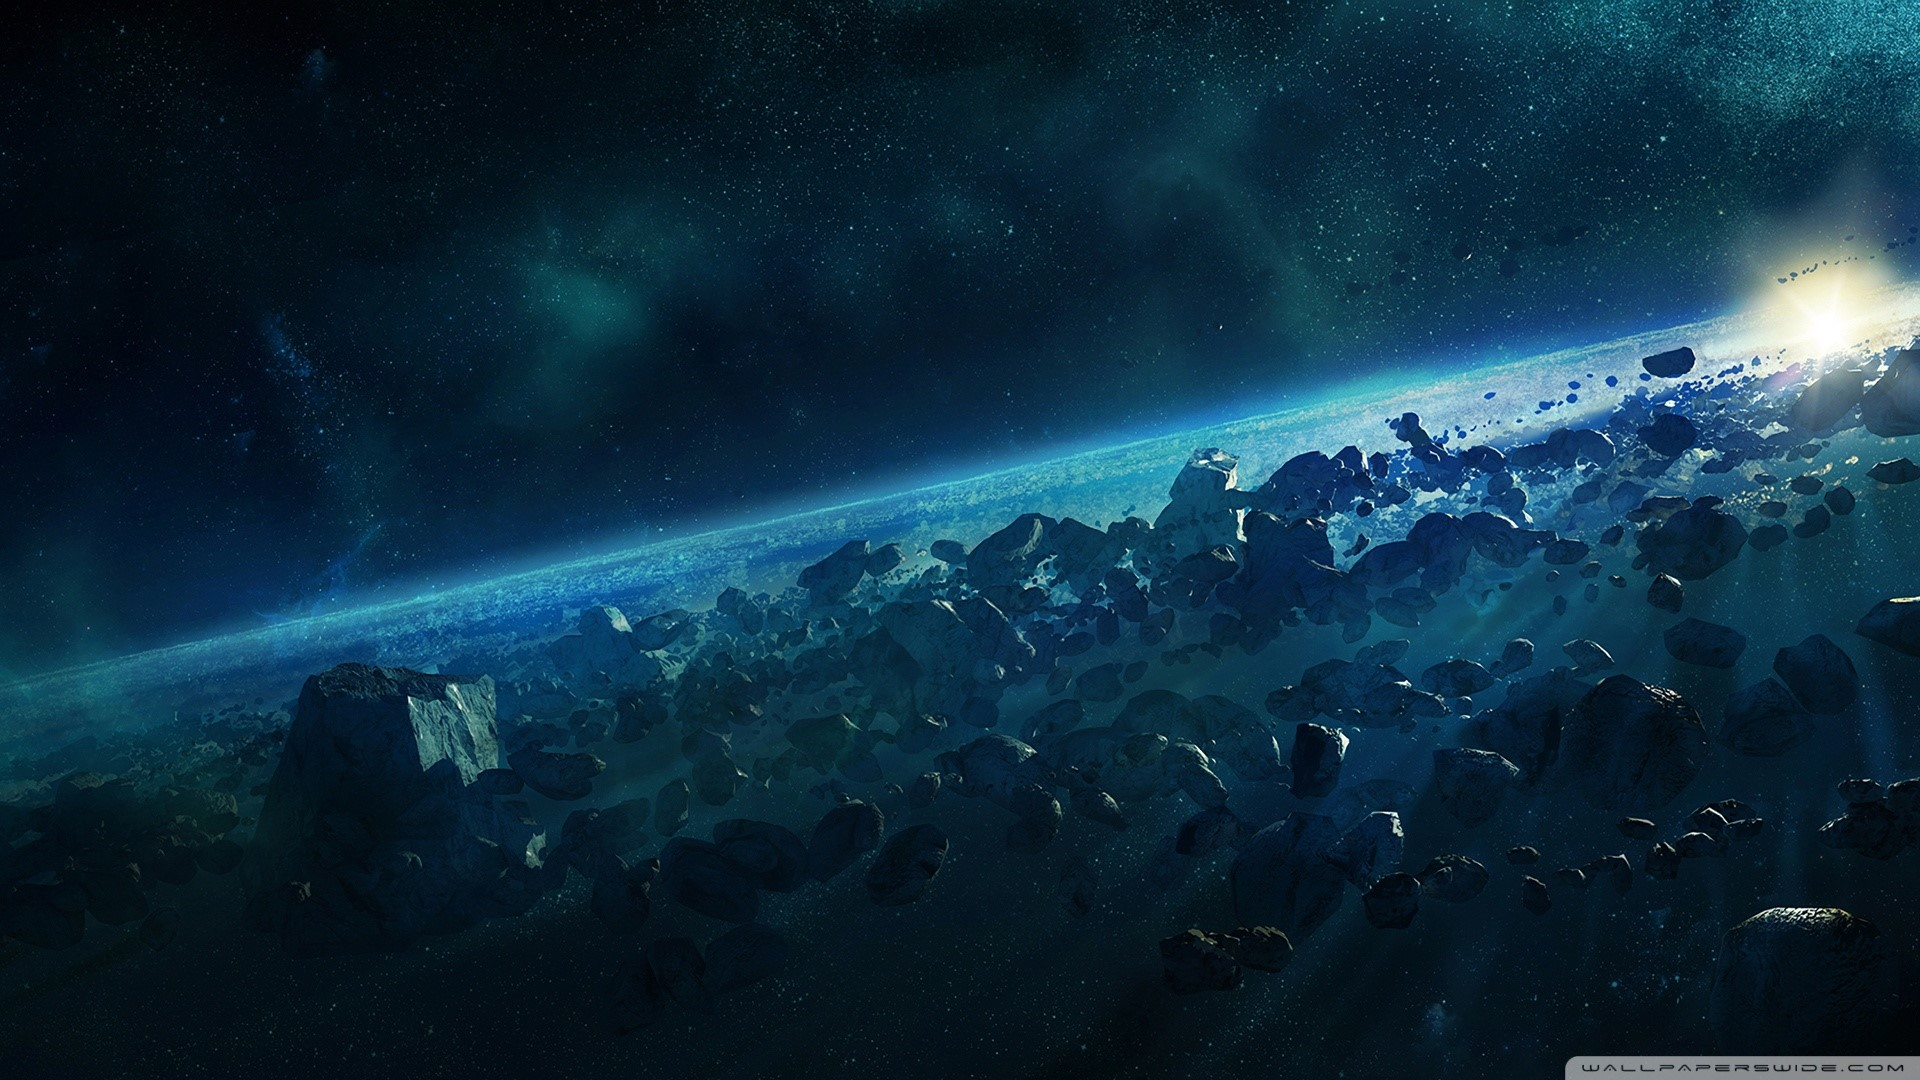
\includegraphics[width=\paperwidth]{Pic/Intro.jpg}}
\title[AMS project]{ Stationary states of opinion diffusion}
\subtitle{Project for the exam: AMS (DSE)}
\author{Paola Serra and Marzio De Corato }
\date{\today}

\begin{document}

\begin{frame}
\vspace{+4.2 cm}  \titlepage
\end{frame}

\usebackgroundtemplate{ } 

% Uncomment these lines for an automatically generated outline.
%\begin{frame}{Outline}
%\setcounter{tocdepth}{1}
%\begin{center}
%  \tableofcontents
%\end{center}
%\end{frame}

\section{Intro}

\begin{frame}{Introduction}


\end{frame}

\section{Theoretical framework}

\begin{frame}{}
\begin{center}
{\Huge Ising model}
\end{center}
\end{frame}


\begin{frame}{Ising model}

\begin{itemize}
\item Historical model: an array of spins (e.g.  atoms that can take states $\pm$ 
\end{itemize}

\end{frame}






\begin{frame}[t,allowframebreaks]
\frametitle{Bibliography}
\printbibliography
\end{frame}


\section{Supporting Info}

\subsection{ROC and $\phi$ factor}
\begin{frame}{}
\begin{center}
{\Huge ROC and $\phi$ factor}
\end{center}
\end{frame}






\end{document}
